\documentclass[../TDTM3.tex]{subfiles}%

\begin{document}
\section[s]"2"{Utilisation de la méthode intégrale}
\enonce{%
	À température élevée et en phase gazeuse, le buta-1,3-diène se dimérise en
	4-vinylcyclohexène suivant la réaction totale d'équation
	\[\ce{2C4H6_{\gaz} = C8H12_{\gaz}}\]
	Afin d'étudier cette réaction, une certaine quantité de buta-1,3-diène est
	introduite dans un récipient de volume $V$ constant, maintenu à température
	constante $T = \SI{326}{K}$. On mesure alors la pression partielle en butadiène
	$p_B$ dans le récipient en fonction du temps~:
	\begin{center}
		\begin{tabular}{lcccccccccccc}
			\toprule
			$t(\si{min})$   &
			0               & \num{3.25}  & \num{8.02}  & \num{12.18} & \num{17.3}  & \num{24.55} &
			\num{33.0}      & \num{43.0}  & \num{55.08} & \num{68.05} & \num{90.1}  &
			\num{119}                                                                               \\
			\midrule
			$p_B(\si{bar})$ &
			\num{0.843}     & \num{0.807} & \num{0.756} & \num{0.715} & \num{0.670} &
			\num{0.615}     & \num{0.565} & \num{0.520} & \num{0.465} & \num{0.423} &
			\num{0.366}     & \num{0.311}                                                           \\
			\bottomrule
		\end{tabular}
	\end{center}
}

\QR{%
	Montrer, en utilisant la loi des gaz parfaits, que la connaissance de
	la pression initiale $p_B$ et de la température $T$ suffit pour calculer
	la concentration initiale $c_B$ en buta-1,3-diène.
}{%
	On utilise la loi du gaz parfait~:
	\begin{gather*}
		\frac{n_B}{V} = \frac{p_B}{RT}
		\Leftrightarrow
		\boxed{c_B = \frac{p_{B,0}}{RT}}
		\qavec
		\left\{
		\begin{array}{rcl}
			p_{B,0} & = & \SI{0.843}{bar} = \SI{8.43e-4}{Pa} \\
			R       & = & \SI{8.314}{J.mol^{-1}.K^{-1}}      \\
			T       & = & \SI{326}{K}
		\end{array}
		\right.\\
		\mathrm{A.N.~:}\quad
		\boxed{c_B = \SI{31.5}{mol.m^{-3}}}
		\Leftrightarrow
		\boxed{c_B = \SI{31.5e-3}{mol.L^{-1}}}
	\end{gather*}
	Faites bien attention aux unités utilisées dans l'application numérique,
	qui viennent ici de celles de l'équation d'état des gaz parfait.
}

\QR{%
Montrer que les résultats sont compatibles avec une cinétique d'ordre
2. Déterminer alors la constante de vitesse à cette température.
}{%
Faisons l'hypothèse d'une cinétique d'ordre 2. Pour simplifier les
écritures, notons $\ce{X} = \ce{C4H6}$. Une loi de vitesse d'ordre 2 en
X signifie qu'elle s'écrit
\[
	v = k[\ce{X}]^2
	\qquad\text{mais on a aussi}\qquad
	v = - \frac{1}{2} \dv{[\ce{X}]}{t}
\]
grâce au lien entre vitesse de disparition d'un réactif et vitesse d'une
réaction. Avec une séparation des variables, cela se traduit par
\begin{gather*}
	- \frac{1}{2} \dv{[\ce{X}]}{t} = k[\ce{X}]^2
	\Leftrightarrow
	\frac{\mathrm{d} [\ce{X}]}{[\ce{X}]^2} = -2k\dt
	\Leftrightarrow
	- \frac{1}{[\ce{X}]} = -2kt + K
\end{gather*}
en primitivant de part et d'autre. On trouve $K$ par la condition
initiale~: $[\ce{X}](t=0) = c_{B,0}$. On a donc \fbox{$K = -1/c_{B,0}$}
et finalement
\[\boxed{ \frac{1}{[\ce{X}]} = \frac{1}{c_{B,0}} + 2kt}\]
Pour vérifier cet ordre 2, il suffit donc de tracer

\begin{minipage}{0.45\linewidth}
	\[  y = ax + b
		\qavec
		\left\{
		\begin{array}{rcl}
			y        & = & \frac{1}{[\ce{X}]} \\\relax
			[\ce{X}] & = & \frac{p_B}{RT}     \\
			a        & = & 2k                 \\
			x        & = & t                  \\
			b        & = & \frac{1}{c_{B,0}}
		\end{array}
		\right.
	\]
\end{minipage}
\begin{minipage}{0.55\linewidth}
	\begin{center}
		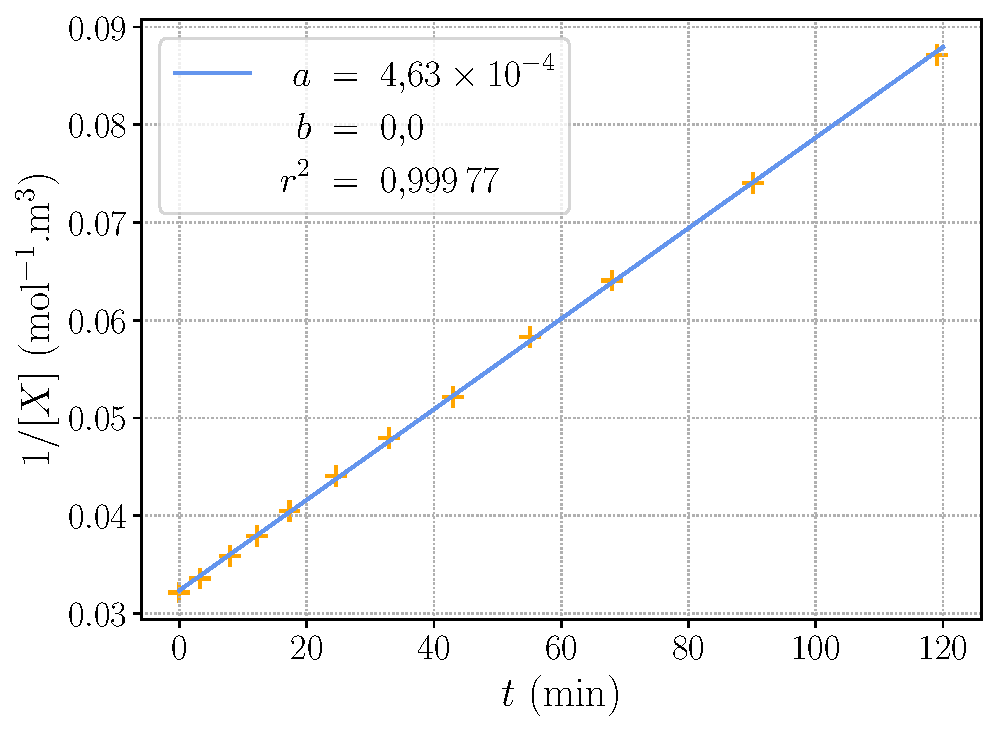
\includegraphics[width=\linewidth]{exo2_x}
	\end{center}
\end{minipage}
On observe que la régression passe bien par tous les points, et on
trouve également $r^2 = \num{0.9997}$, validant l'ordre 2. Le
coefficient directeur valant $2k$, on trouve finalement
\[\boxed{k =
	\SI{2.32e-4}{mol^{-1}.m^3.min^{-1}}
	=
	\SI{2.32e-1}{mol^{-1}.L.min^{-1}}
	}
\]
}

\QR{%
	Déterminer le temps de demi-réaction du système précédent.
}{%
	Pour un système d'ordre 2, on a $t_{1/2} = \frac{1}{ka[\ce{A}]_0}$ avec
	$a$ le coefficient stœchiométrique arithmétique de l'élément A. Ici, le
	coefficient stœchiométrique du butadiène est 2, et on a donc
	\begin{gather*}
		t_{1/2} = \frac{1}{2kc_{B,0}}
		\Leftrightarrow
		\boxed{t_{1/2} = \SI{70.0}{min}}
	\end{gather*}
}
\QR{%
	On admet souvent qu'une réaction est pratiquement terminée lorsque au
	moins 99\% du réactif limitant a été consommé. Déterminer la durée
	d'évolution du système précédent~; exprimer cette durée en fonction du
	temps de demi-réaction.
}{%
	On cherche donc $t_{99}$ tel qu'il ne reste que 1\% de $c_{B,0}$,
	c'est-à-dire~:
	\begin{gather*}
		[\ce{X}](t = t_{99}) = \frac{1}{100}c_{B,0}
		\Leftrightarrow
		\frac{100}{c_{B,0}} = \frac{1}{c_{B,0}} + 2kt_{99}
		\Leftrightarrow
		t_{99} = \frac{1}{2k}\times \frac{99}{c_{B,0}}\\
		\Leftrightarrow
		\boxed{
			t_{99} = 99t_{1/2}
		}
		\qdonc
		\boxed{t_{99} = \SI{6930}{min} = \SI{115.5}{h} = \SI{4.8125}{jours}}
	\end{gather*}
}
\end{document}
